\documentclass{beamer}
\usepackage[italian]{babel}
\usepackage{amsmath}
\usepackage{amsthm}
\usepackage{amssymb}
\usepackage{amscd}
\usepackage{amsfonts}
\usepackage{booktabs}
\usepackage{enumerate}
\usepackage{array}
\usepackage{comment}
\usepackage{animate}
\usepackage{graphicx}
\usepackage{adjustbox}
\usepackage{tcolorbox}
\usepackage[algo2e]{algorithm2e}
\usepackage{bm}
\usepackage{subfig}
\usepackage{tikz}
\usepackage{xcolor}
\usepackage{commath}
\usepackage{siunitx}
\usepackage{physics}
\usepackage{wrapfig}

\setlength{\parskip}{5pt}%
\setlength{\columnsep}{1pt}%

\newcommand{\ca}{\text{Ca}^{2+}}

\usepackage{etoolbox} %Chiama la barra del titolo anche senza inserire il titolo slide
%
% Choose how your presentation looks.
%
% For more themes, color themes and font themes, see:
% http://deic.uab.es/~iblanes/beamer_gallery/index_by_theme.html
%
\mode<presentation>
{
  \usetheme[nologos]{Padova}      % or try Darmstadt, Madrid, Warsaw, ...
  \usecolortheme{default} % or try albatross, beaver, crane, ...
  \usefonttheme{default}  % or try serif, structurebold, ...
  \setbeamertemplate{navigation symbols}{}
  \setbeamertemplate{caption}[numbered]
} 

% \usepackage[utf8]{inputenc}
% \usepackage[T1]{fontenc}

\title{Single Channel Kinetics of BK Channels}
\subtitle{A review article by Y. Geng and K. L. Magleby}
\author{Giorgio Palermo}
\date{08/07/2020}
\institute{LM Physics - a.a. 2019/20 - Biological Physics }

\begin{document}

\begin{frame}{}
  \titlepage
\end{frame}

\begin{frame}
\frametitle{Table of Contents}
\tableofcontents
\end{frame}

\section{Introduction}

\begin{frame}{Introduction}
\begin{minipage}{.4\textwidth}
\begin{figure}
\centering
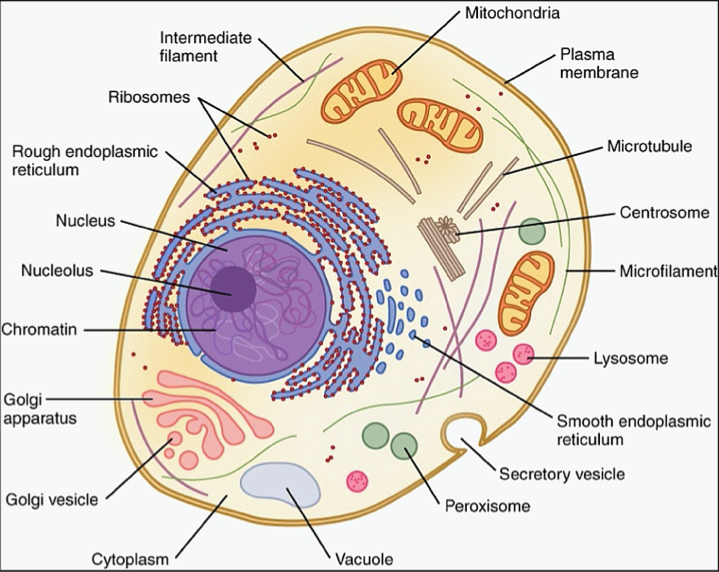
\includegraphics[width=\textwidth]{Cell_Cartoon.png}
\end{figure}
\end{minipage}
\hfill
\begin{minipage}{.5\textwidth}
\begin{figure}
\centering
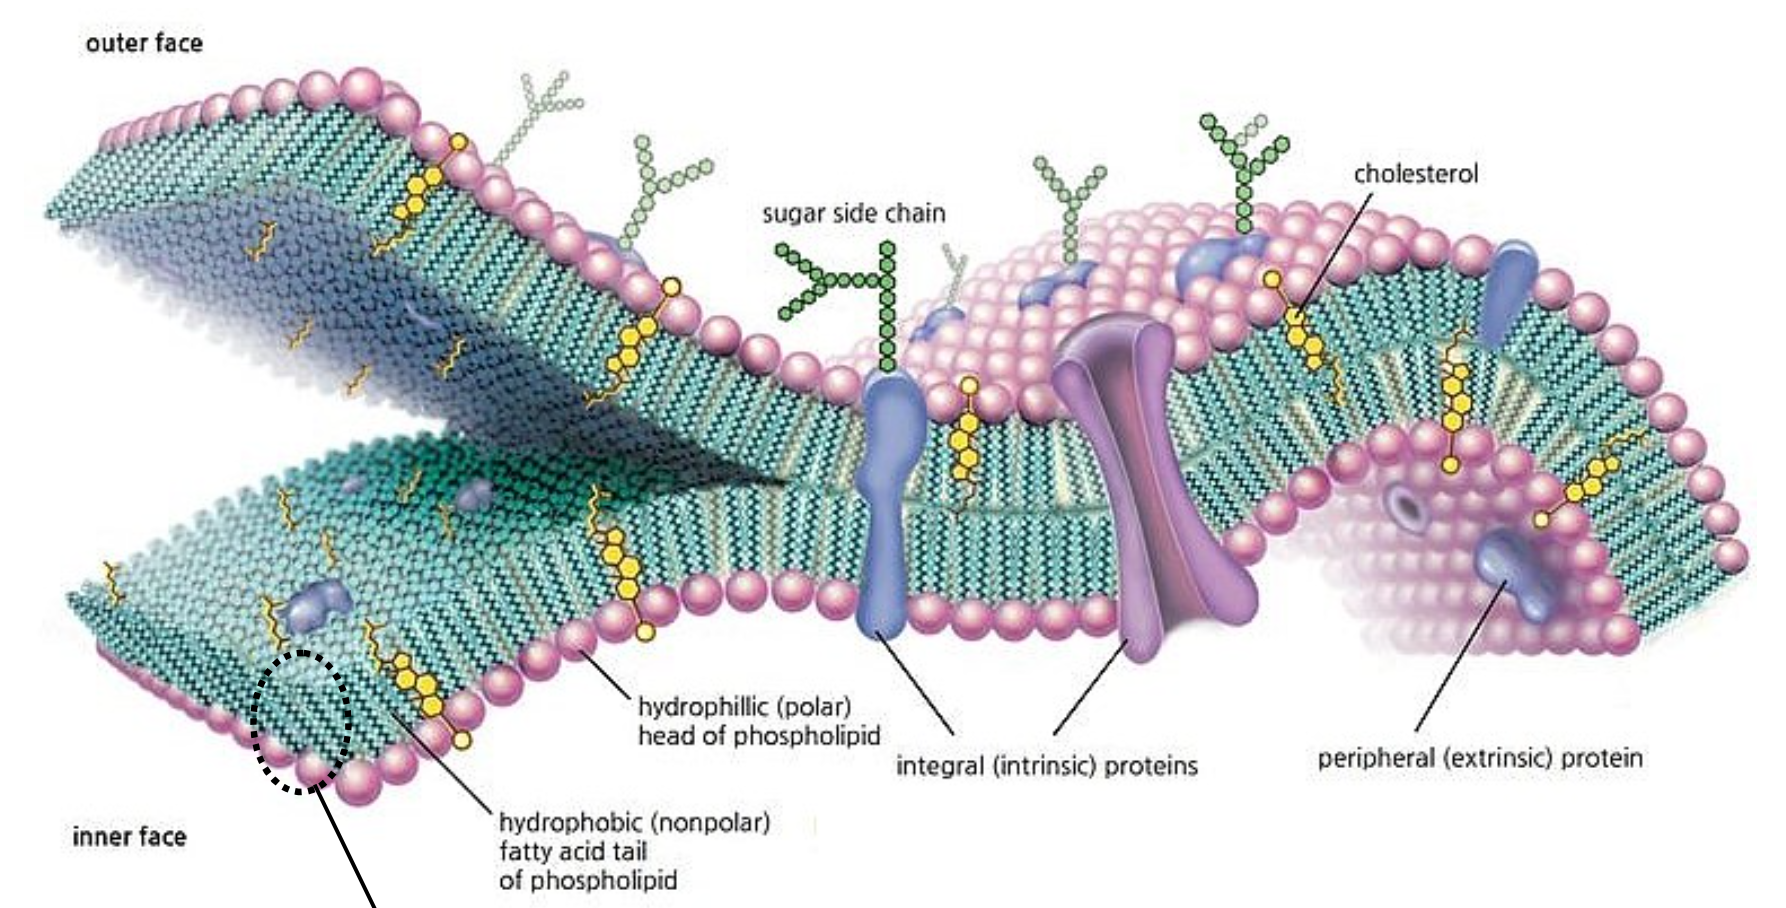
\includegraphics[width=\textwidth]{Cell_Membrane.png}
\end{figure}
\end{minipage}

\begin{figure}
\centering
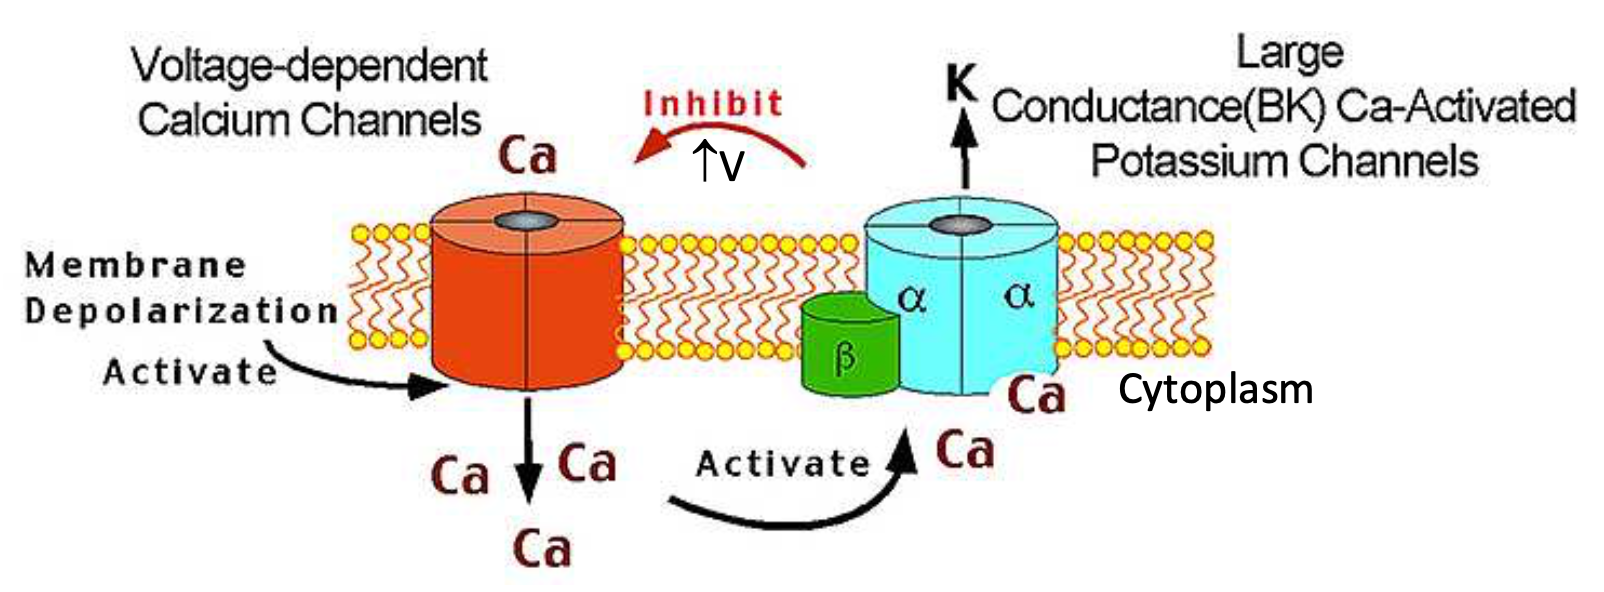
\includegraphics[width=.8\textwidth]{Feedback_Mechanism.png}
\end{figure}
\end{frame}

\section{BK channel: modular structure}

\begin{frame}{Structure of a BK channel}
\begin{figure}
\centering
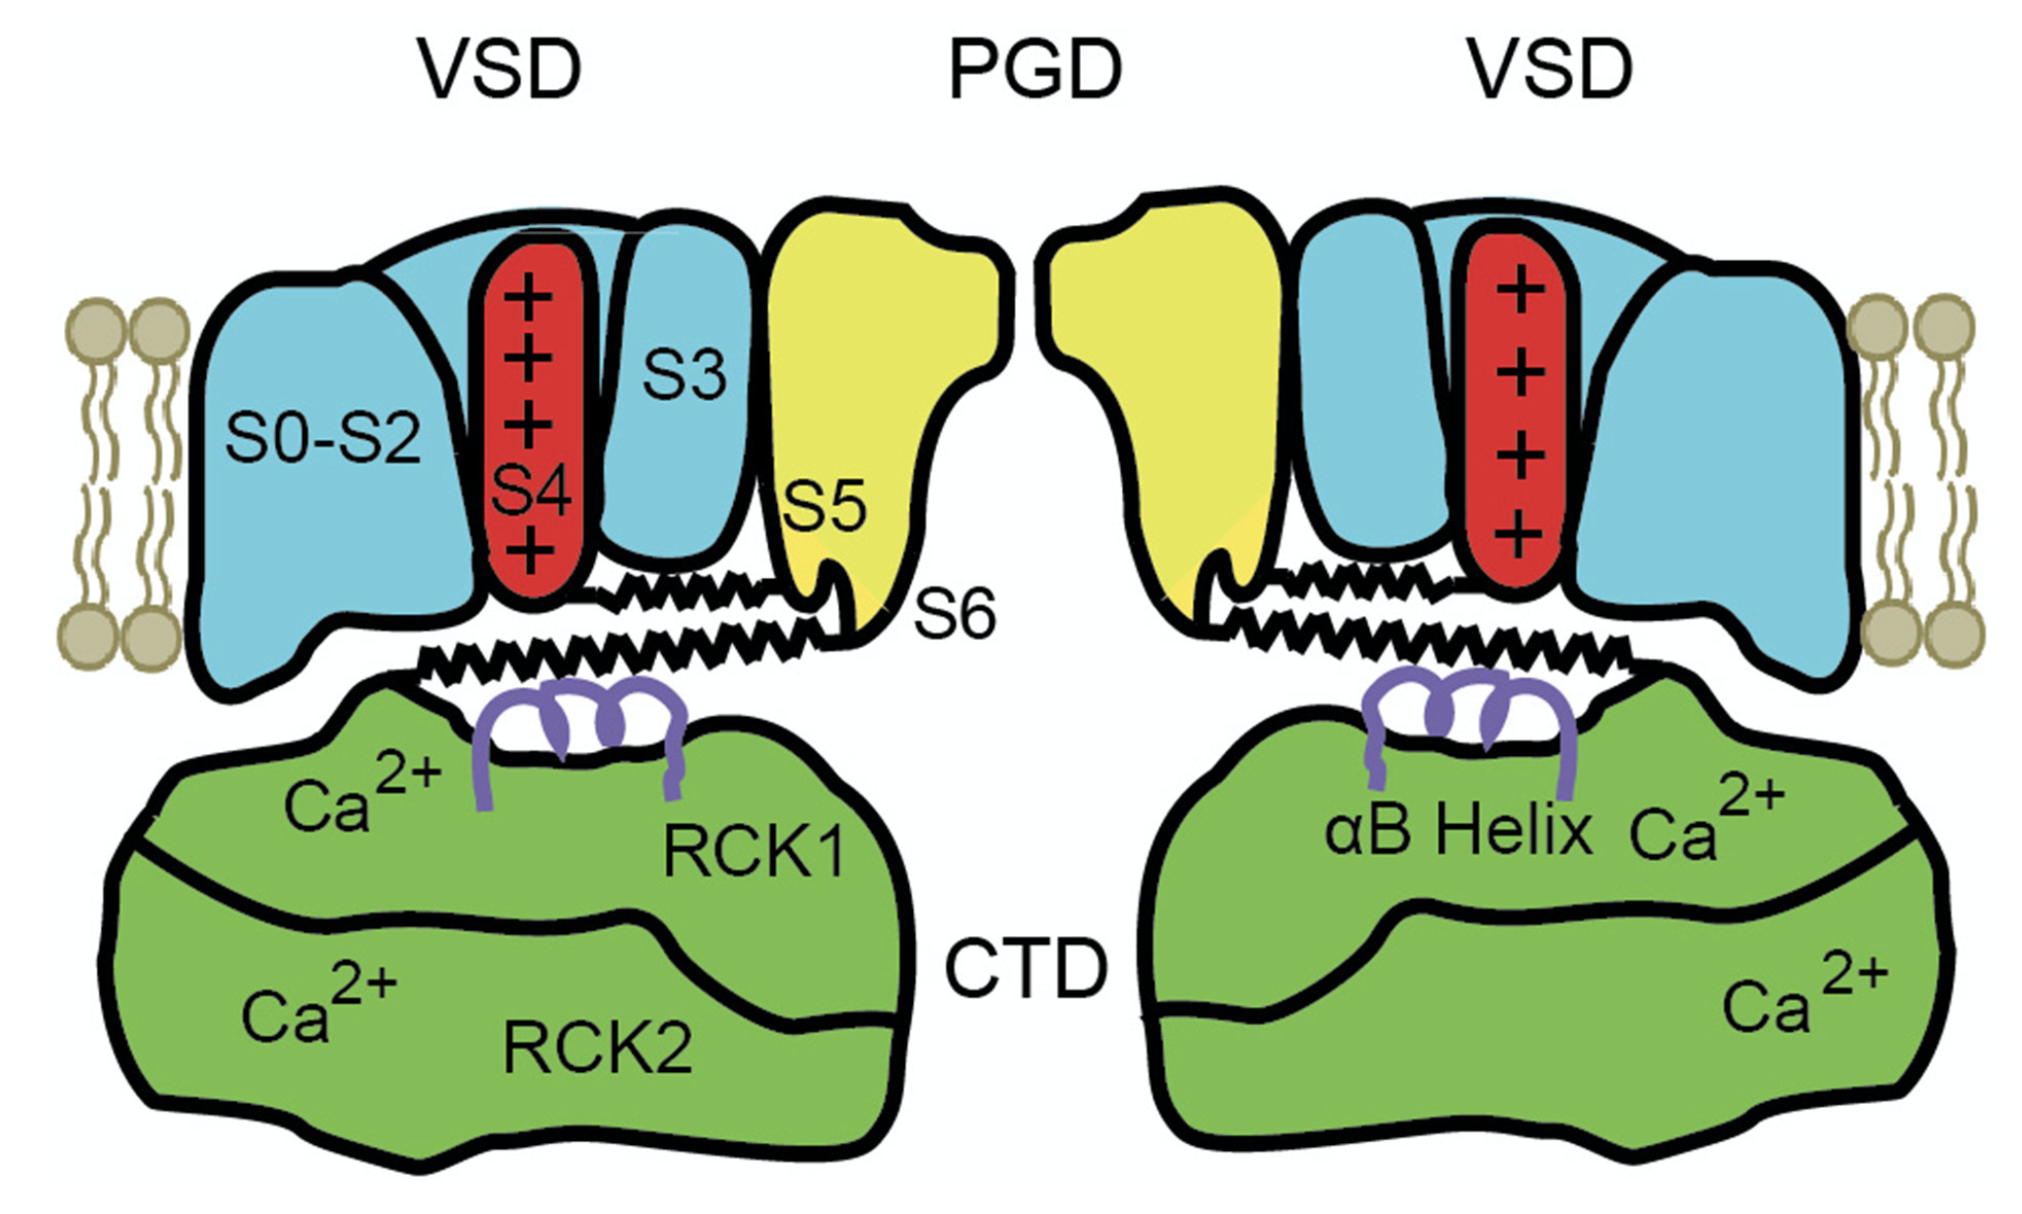
\includegraphics[width=.8\textwidth]{BK_Cartoon.png}
\end{figure}
\hfill
\end{frame}

\section{DSM and gating mechanism}
\begin{frame}[t]\frametitle{DSM models}
    DSM stands for \emph{Discrete State Markov.}

    Idea: channels gate by moving among conformational states: $\rightarrow \quad\{\# \text{VSDs};\ \# \text{RCKs};\ \text{O/C PGD}\}$

    Dwell-times $\tau$: exponentially distributed.

    If gating concerns more than two states: $\quad \tau_i = \frac{1}{\sum_{j\neq i} k_{i\rightarrow j}}$
  
    with $k_{i\rightarrow j}$ rate constant for transition from state $i$ to state $j.$


    Crucial assumptions for DSM for BK channels:
	\begin{itemize}
    	\item Short transition times: irrelevant w.r.t. open/closed times
    	\item Rate constants invariant for constant experimental condition
    	\item The gating takes place by means of changing the rate constants
    \end{itemize}



\end{frame}

\begin{frame}{Gating mechanism (I)}
The theoretical structure of a gating mechanism has to be formulated according to what is known about the microscopic structure of the considered ion channel.

The BK channel structure is made of:
\begin{itemize}
	\item PGD
	\item Four VSDs
	\item Four pairs of RCK domains
\end{itemize}

States of the model $ \quad \leftrightarrow \quad\{\# \text{VSDs};\ \# \text{RCKs};\ \text{O/C PGD}\}$
 
Observations say that voltage and $\ca$ activation systems of BK channels are (mainly) independent $\rightarrow$ the starting point is to build separate models for each.
\end{frame}

\begin{frame}{Gating mechanism (II)}
\begin{minipage}{.46\textwidth}
Voltage gating:
\begin{itemize}
	\item each state can be open or closed
	\item each VSD can be activated/deactivated
\end{itemize}
\bigskip
$\ca$ gating:
\begin{itemize}
	\item each state can be open or closed
	\item each RCK can be bound/unbound to $\ca$
\end{itemize}
\end{minipage}
\begin{minipage}{.52\textwidth}
\begin{figure}
\centering
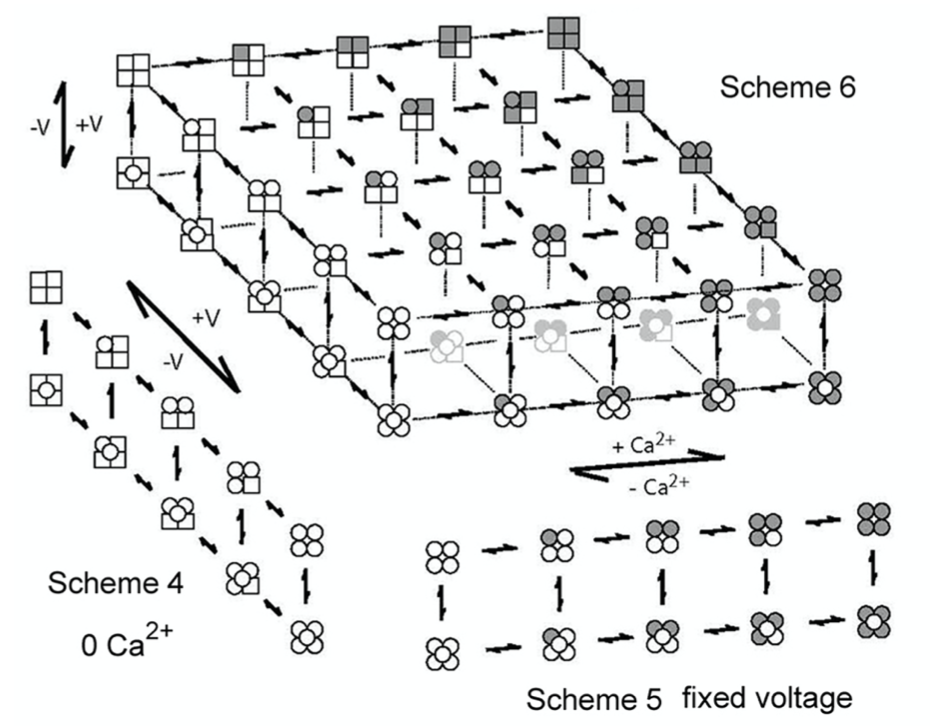
\includegraphics[width=\textwidth]{50_State_Model.png}
\end{figure}
\end{minipage}
\end{frame}

\begin{frame}{Gating mechanism (III)}
\begin{minipage}{.46\textwidth}
\begin{itemize}
	\item Voltage gating $\rightarrow$ 10-state model

	\item $\ca$ gating $\rightarrow$ 10-state model
\end{itemize}
\bigskip
$\implies$ 25 closed + 25 open states = 50-state model for BK gating.
\end{minipage}
\begin{minipage}{.52\textwidth}
\begin{figure}
\centering
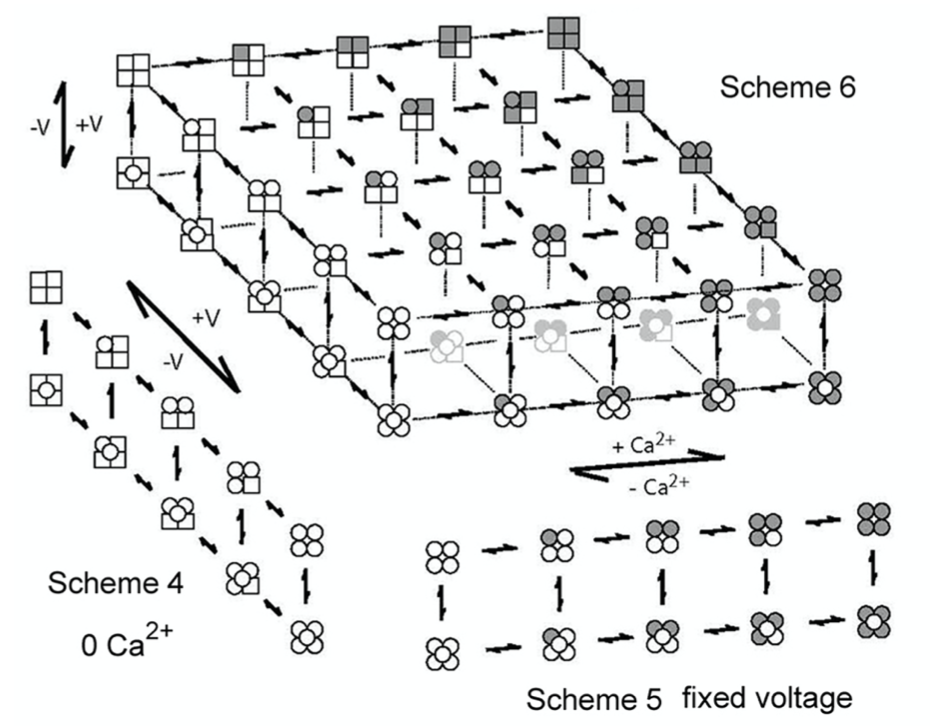
\includegraphics[width=\textwidth]{50_State_Model.png}
\end{figure}
\end{minipage}
\end{frame}



\begin{frame}{Effective number of visited states (I)}
\begin{figure}
\centering
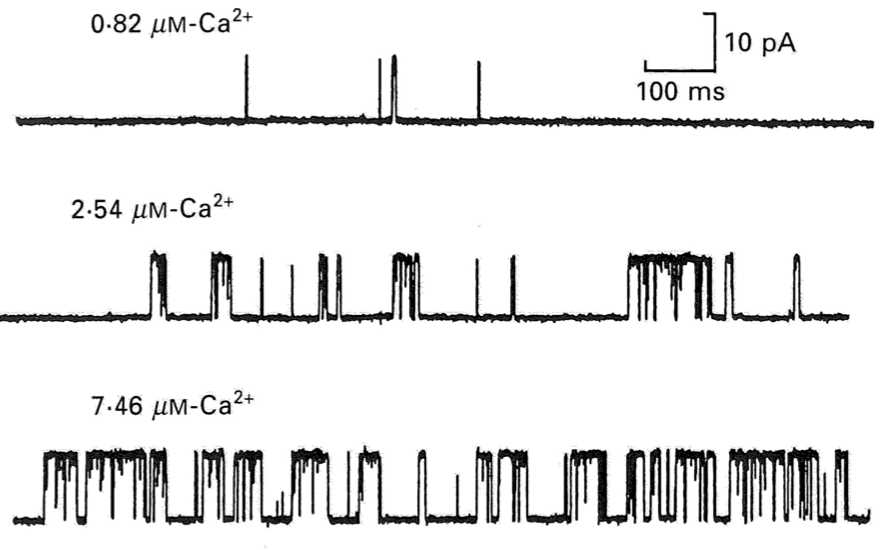
\includegraphics[width=.7\textwidth]{Ca_activation_v_vs_time.png}
\end{figure}

Single channel current recordings at three different $\ca$ concentrations $\rightarrow$ $\ca$ induces increase in channel activity.
\end{frame}

\begin{frame}{Effective number of visited states (II)}
Measuring open and closed interval durations for long records and stable data we can build:
\begin{figure}
\centering
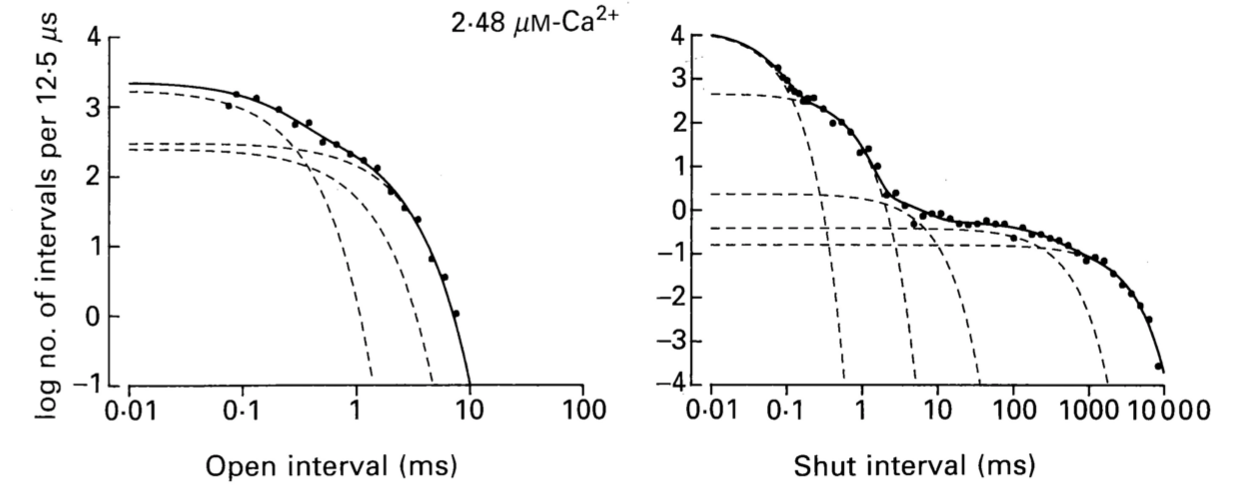
\includegraphics[width=.7\textwidth]{Ca_activation_time_interv_distrib.png}
\end{figure}
Significant exponential components: 3 for open intervals and 5 for closed intervals $\rightarrow$ clue of the minimum number of states over which the gating is taking place.

Why not 25 open and 25 closed states?

\end{frame}

\begin{frame}{Effective number of visited states (III)}
\begin{figure}
\centering
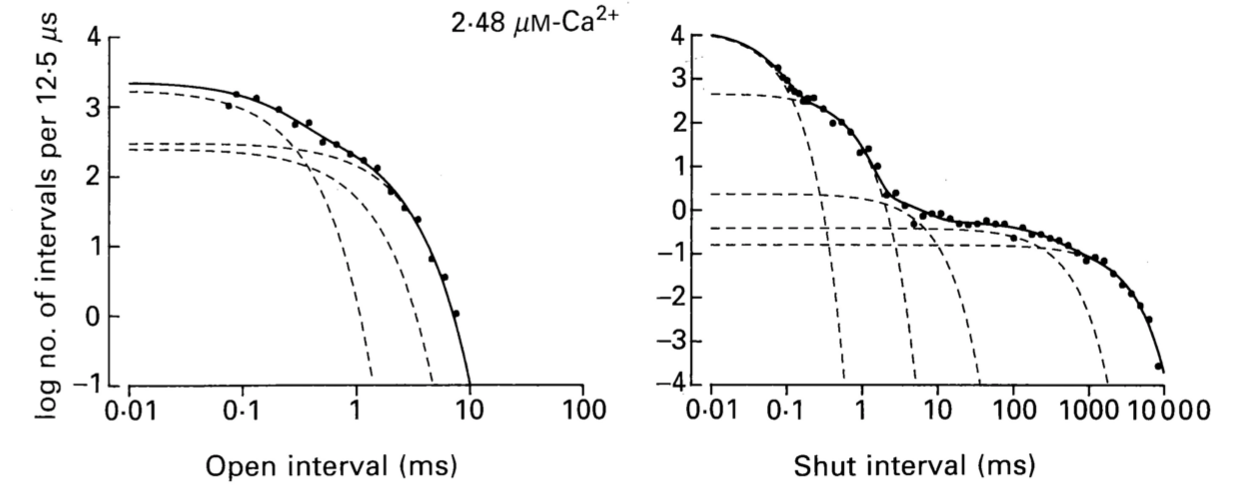
\includegraphics[width=.7\textwidth]{Ca_activation_time_interv_distrib.png}
\end{figure}
Why not 25 open and 25 closed states?
\begin{itemize}
	\item For any fixed voltage and $\ca$ the gating is limited to a small amount of states
	\item Many rate constants for a 50-state model are nearly identical or too close to detect
\end{itemize}

\end{frame}

\section{Results for channel activation}

\begin{frame}{Activation by voltage}
\begin{figure}
\centering
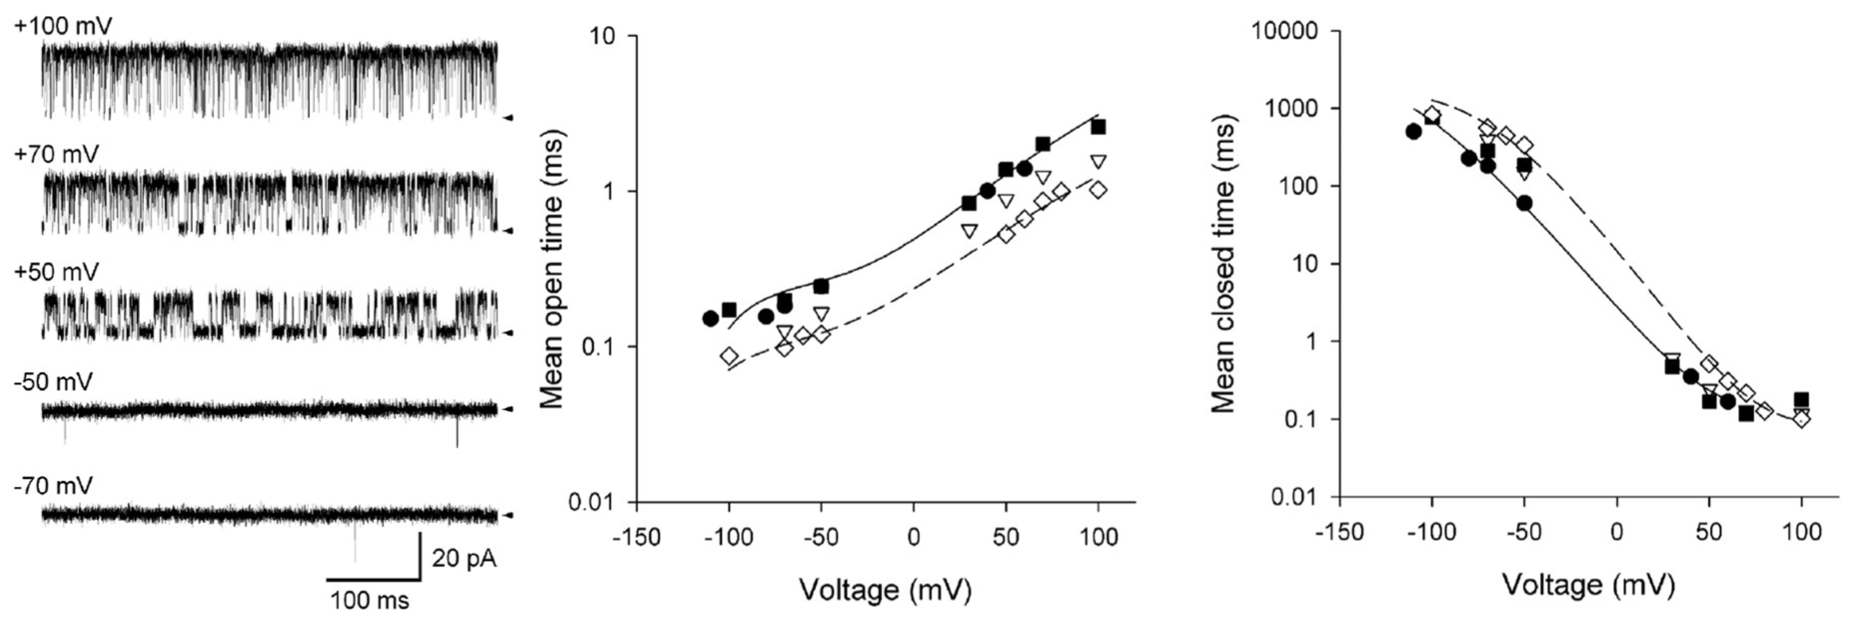
\includegraphics[width=\textwidth]{Voltage_Opening.png}
\end{figure}
Voltage activation from -100 to + 100 mV with $95\ \mu\text{M}\ \ca$ to saturate the $\ca$ sensitive domains.

Mean open interval $\rightarrow$ increased about 12 times;

\vspace{-8pt}
Mean closed interval $\rightarrow$ decreased about 4500 times.
\vfill
\end{frame}

\begin{frame}{Activation by $\ca$}
\begin{figure}
\centering
\includegraphics[width=.9\textwidth]{Ca_activation_1.png}
\end{figure}
\vspace{-5pt}
Activation of a BK channel at the single-channel level by Ca2+, measured at a fixed +30 mV potential.
The dependence of the opening probability on the Ca2+ concentration is steep.

Increasing the $\ca$ from 0.1 to 1000 $\mu\text{M}:$

Mean open interval $\rightarrow$ increased about 10 times;

\vspace{-5pt}
Mean closed interval $\rightarrow$ decreased about 1000 times.
\vfill
\end{frame}

\begin{frame}{Synergistic activation by voltage and $\ca$ (I)}
\begin{figure}
\centering
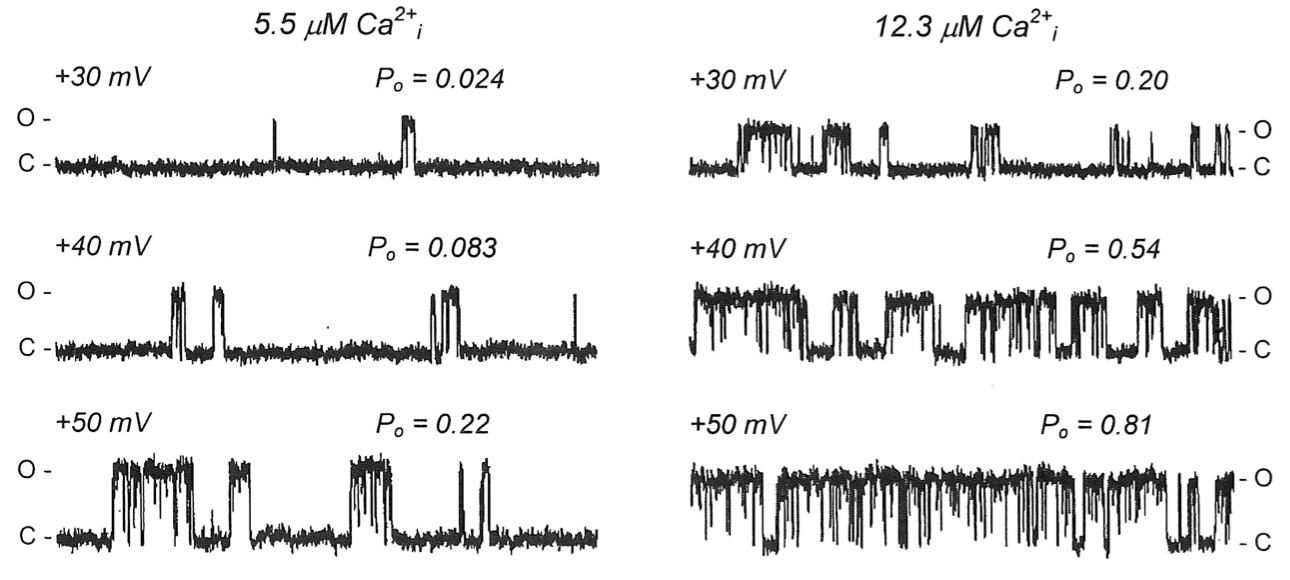
\includegraphics[width=.8\textwidth]{Synergistic_activation_1.png}
\end{figure}
\bigskip
Jointly increasing voltage and $\ca$ leads to synergistic activation of the single channel, increasing the opening probability.
\end{frame}

\begin{frame}{Synergistic activation by voltage and $\ca$ (II)}
\begin{figure}
\centering
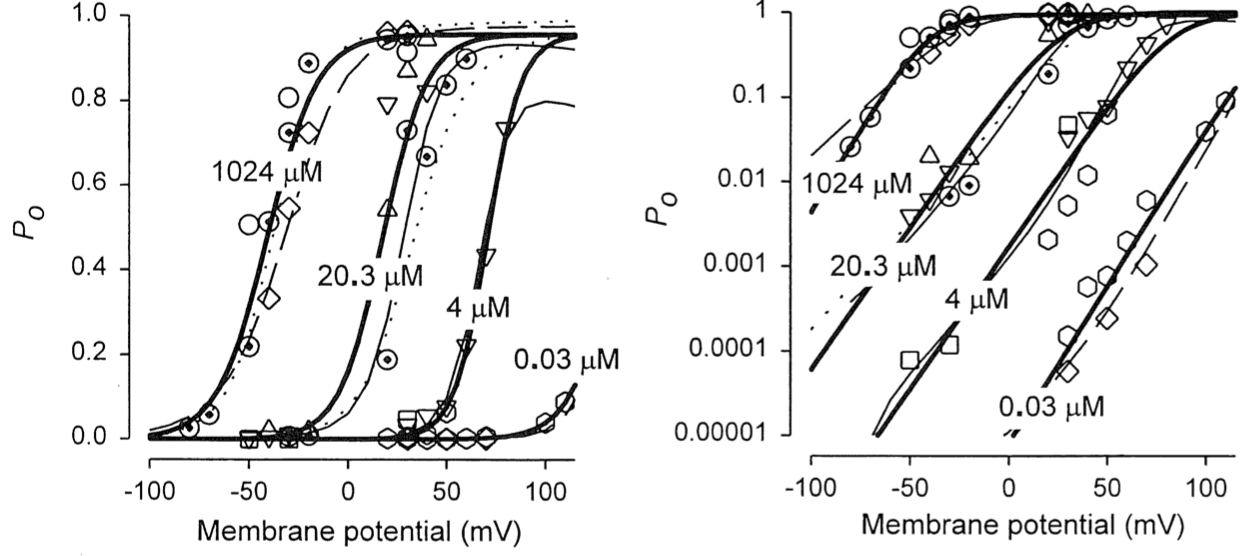
\includegraphics[width=.8\textwidth]{Synergistic_activation_2.png}
\end{figure}

Increasing $\ca$ gives approximately parallel shifts in the opening probability vs. voltage curves, suggesting independent activation by $\ca$ and voltage, consistently with the modular model discussed before (independent mechanisms).
\end{frame}

\begin{frame}{Does the model describe the data?}
\begin{wrapfigure}{R}{0.5\textwidth}
  \begin{center}
    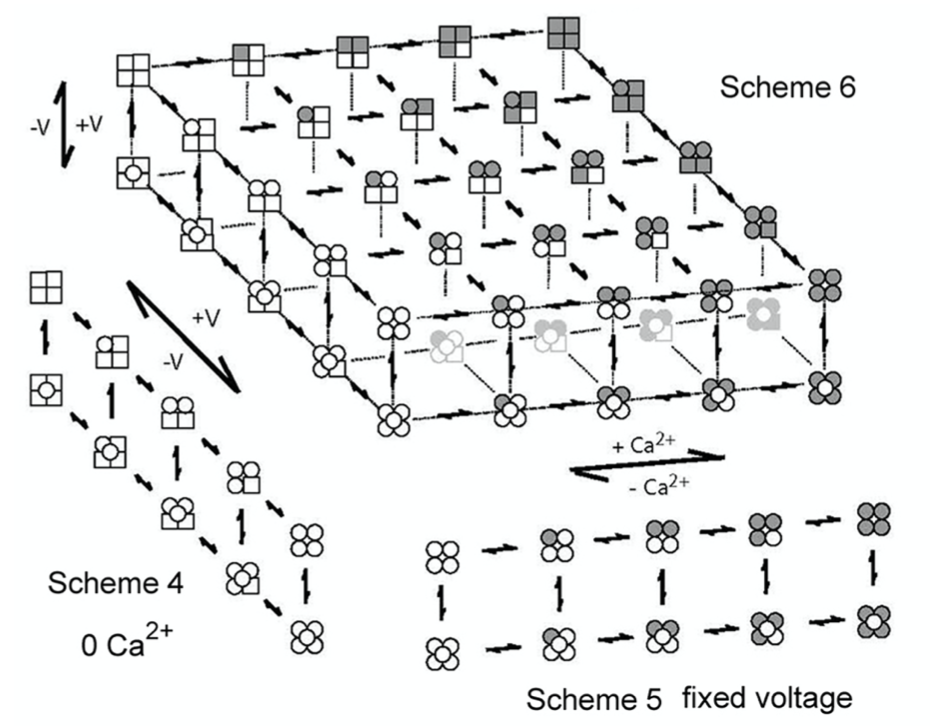
\includegraphics[width=0.38\textwidth]{50_State_Model.png}
  \end{center}
\end{wrapfigure}
Is the 50-state DSM model we derived consistent with the experimental observations?

Tests have been made on restricted models (with reduced number of states), obtaining \emph{good to excellent} agreement with the data.

Restricted models $\rightarrow$ lower number of constants to fit to the data.


$\rightarrow$ 50-state can agree with the data equally or better than one of its sub-models.

\end{frame}

% \begin{frame}{On the action of the gating ring}
% \begin{wrapfigure}{R}{0.5\textwidth}
%   \begin{center}
%     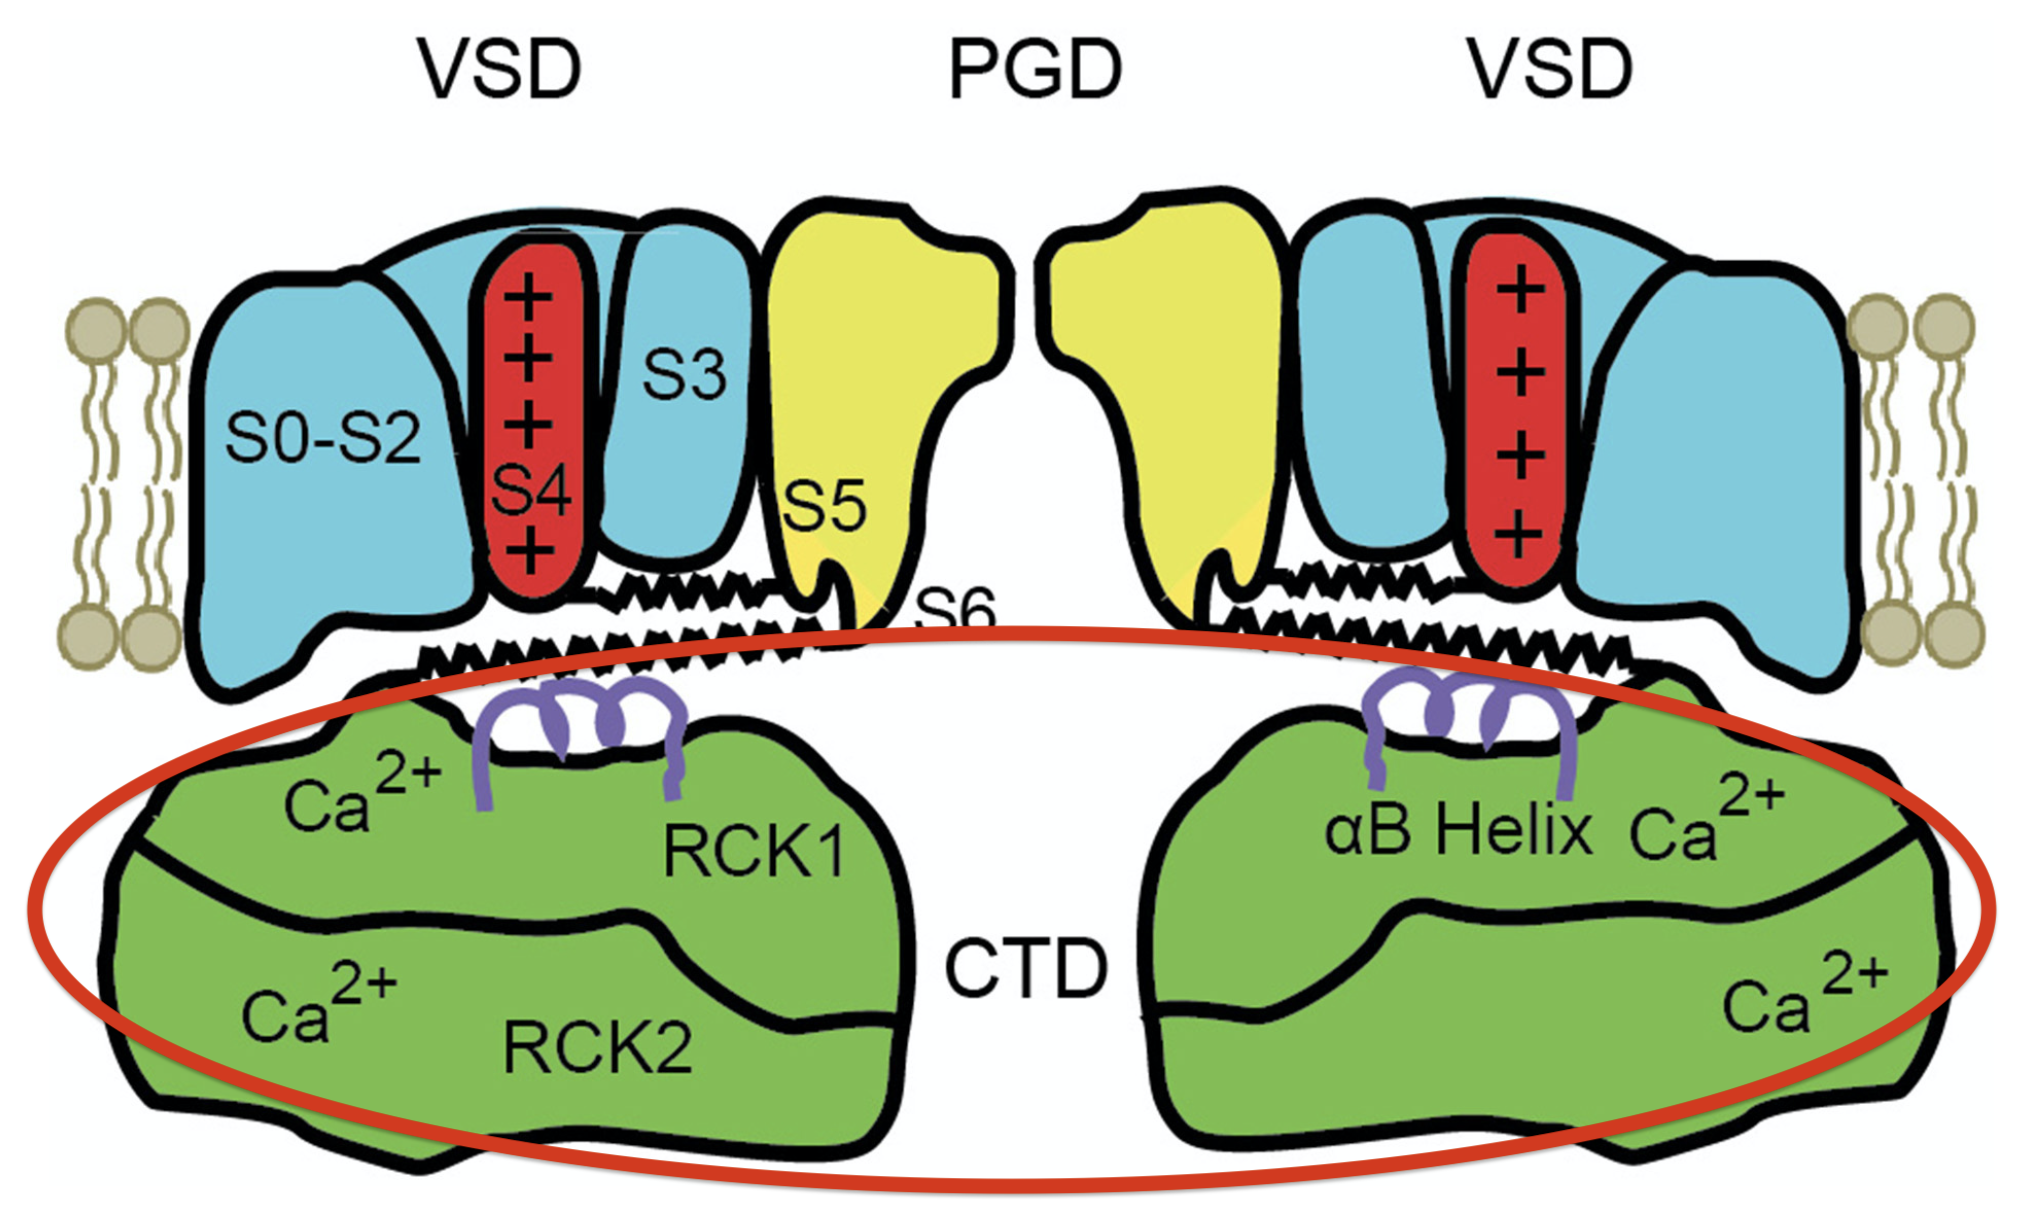
\includegraphics[width=0.38\textwidth]{BK_Cartoon_1.png}
%   \end{center}
% \end{wrapfigure}
% To explore the action of the gating ring and the RCK1-S6 linkers, experiments on mutated BK channels have been made. In particular the mutations involved the absence of the gating ring and the length of the RCK1-S6 linkers.

% It has been shown that the linkers passively pull on the PGD to bias the channel towards opening in absence of Ca2+, while they apply an active opening force in presence of Ca .

% \end{frame}

\begin{frame}[t]{Conclusion}
\begin{figure}
\centering
\subfloat{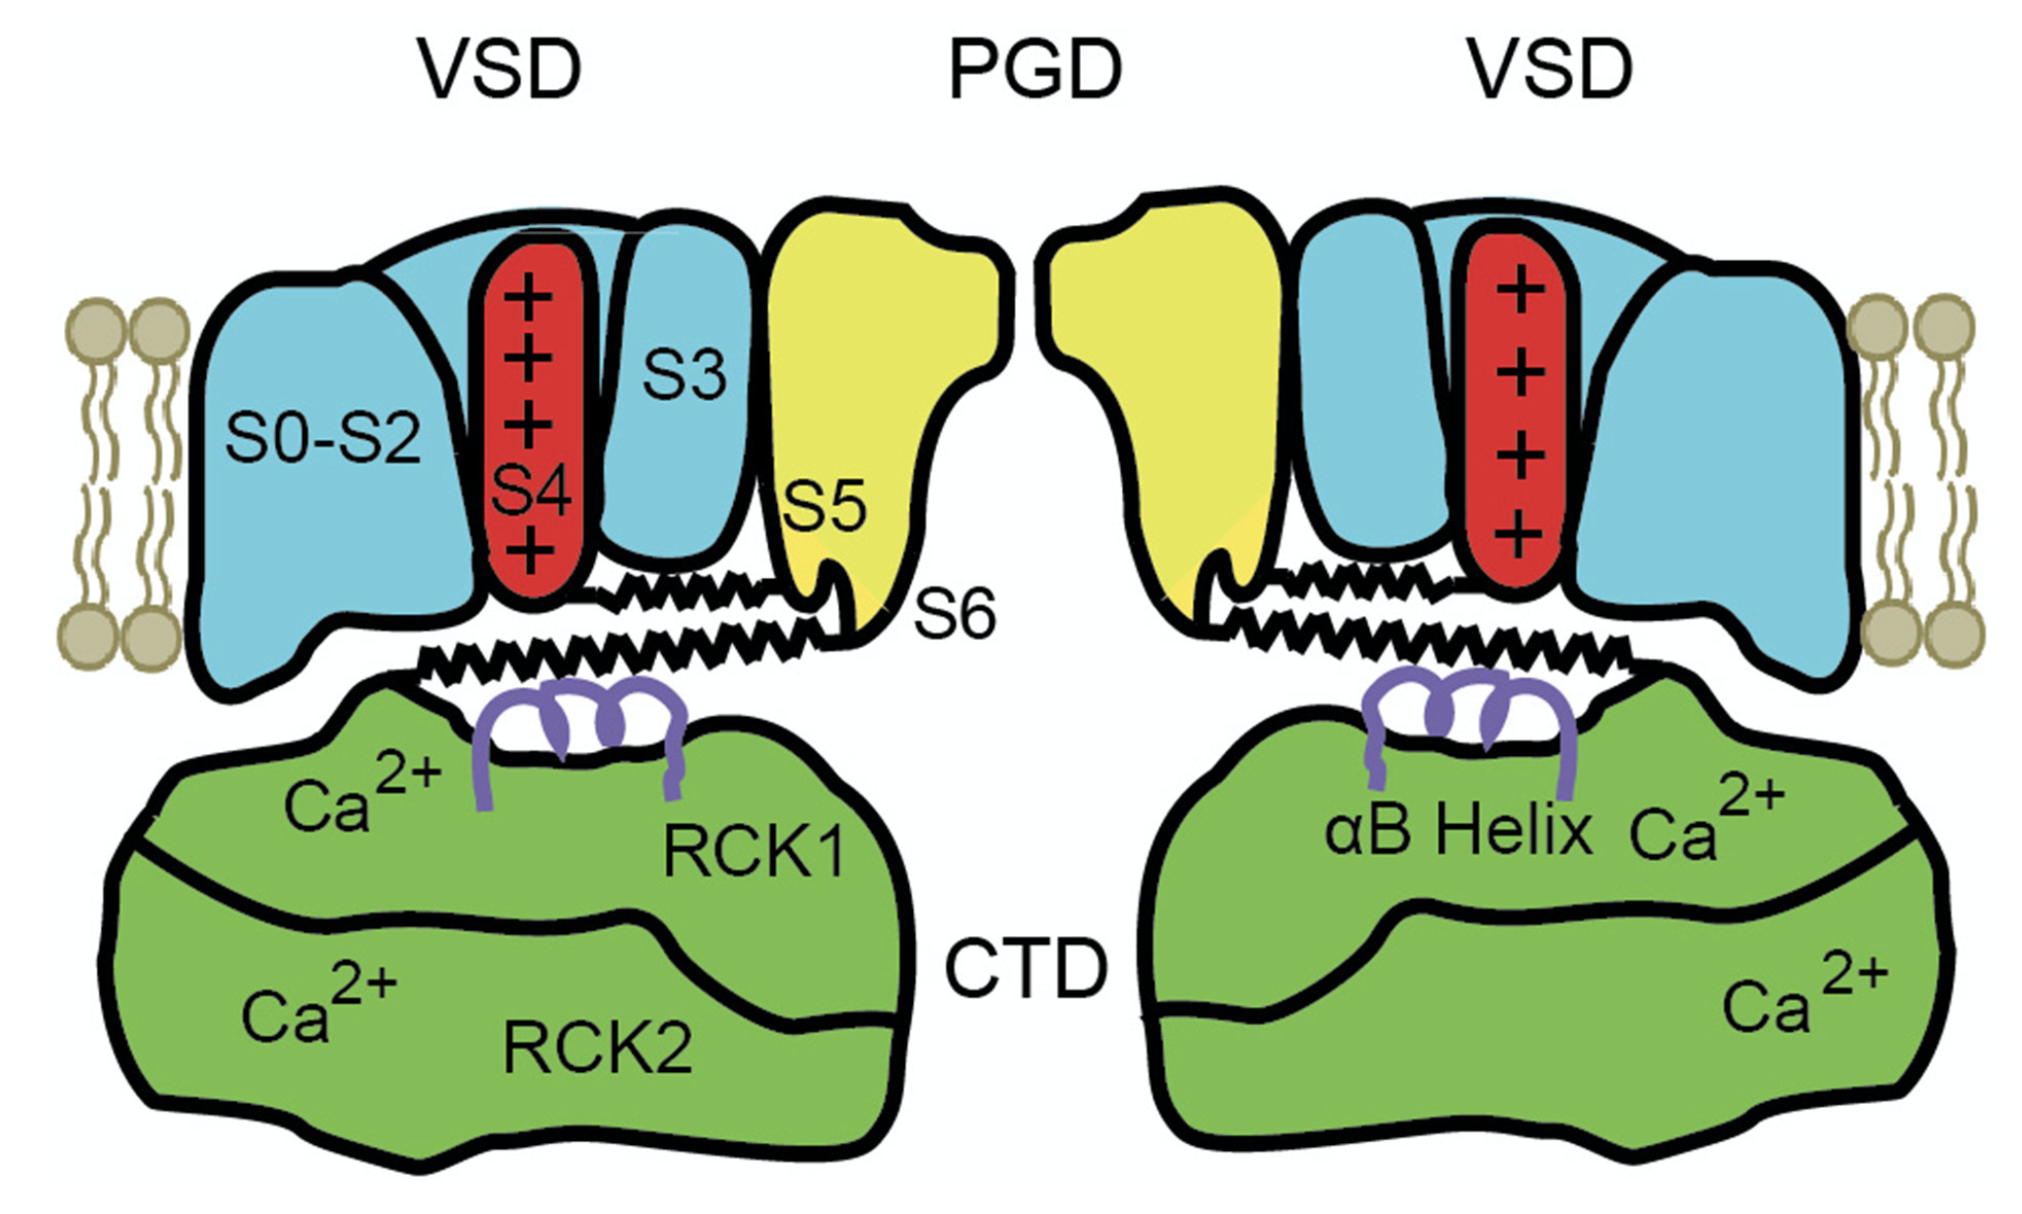
\includegraphics[width=.38\textwidth]{BK_Cartoon.png}}\qquad
\subfloat{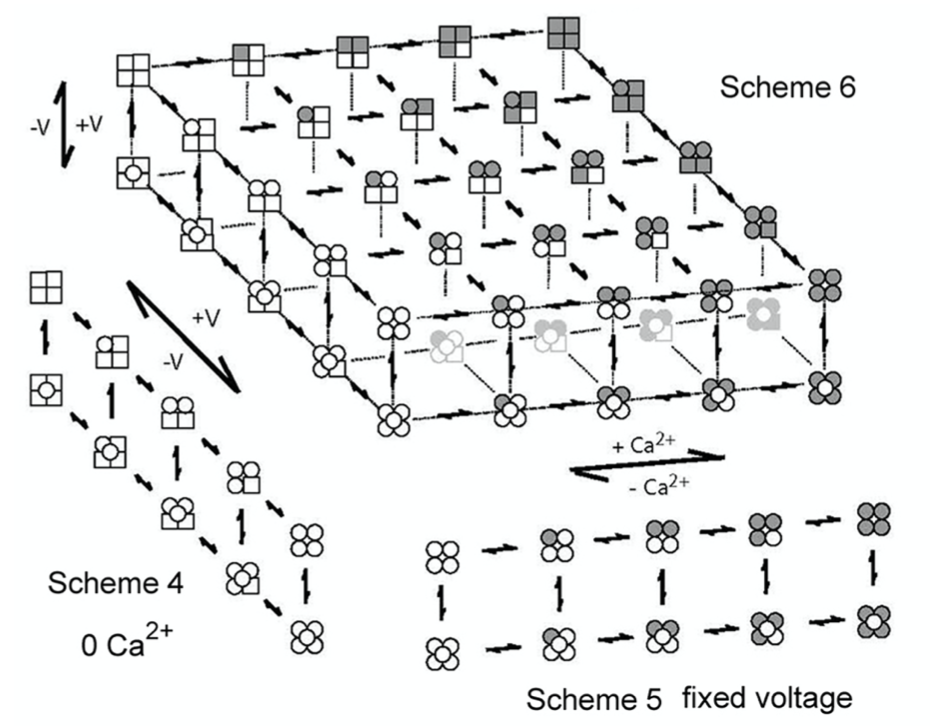
\includegraphics[width=.34\textwidth]{50_State_Model.png}}

\subfloat{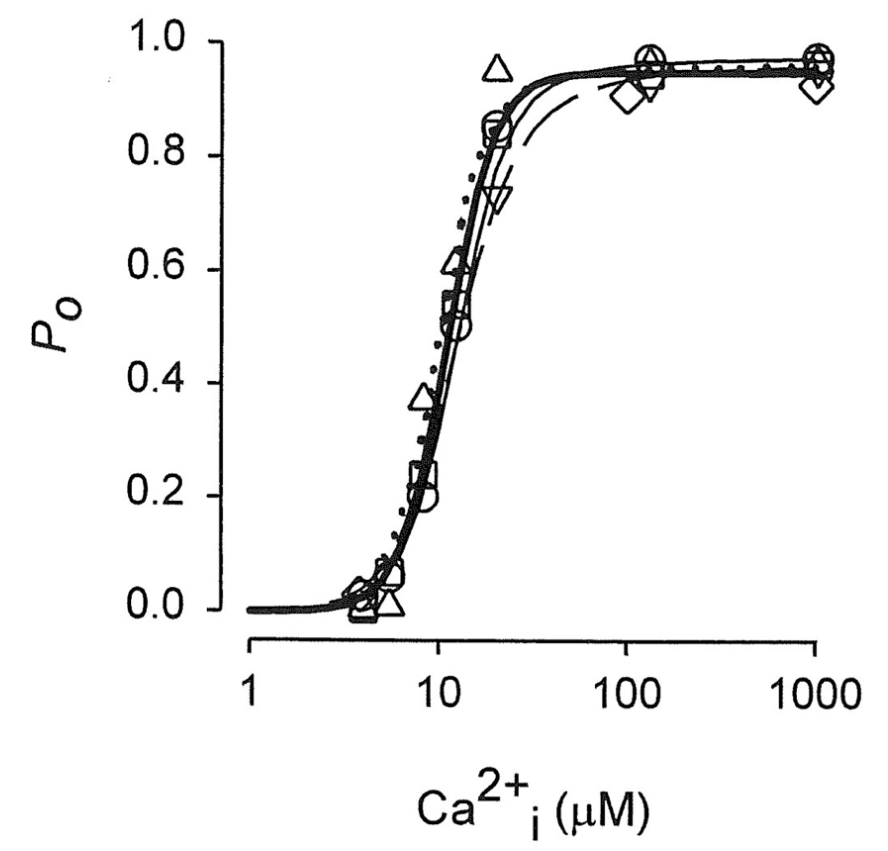
\includegraphics[width=.34\textwidth]{Ca_Activation_Probability.png}}\qquad
\subfloat{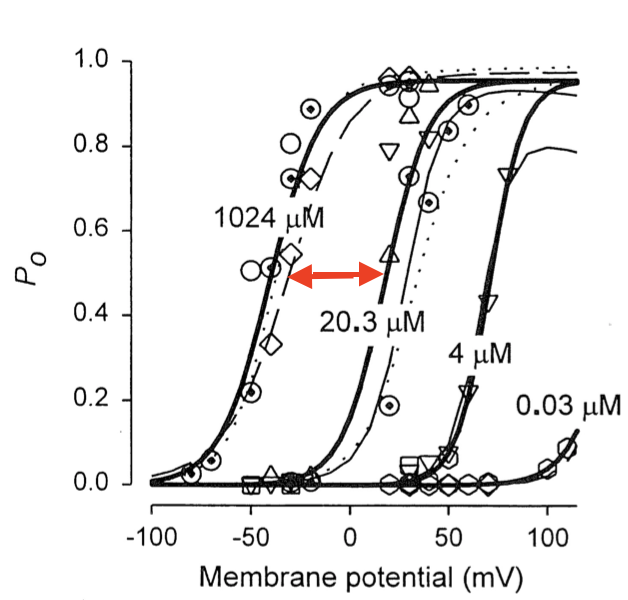
\includegraphics[width=.34\textwidth]{Synergic_Activstion_3.png}}
\vfill
\end{figure}
\end{frame}

\begin{frame}{Conclusion}
\begin{figure}
\centering
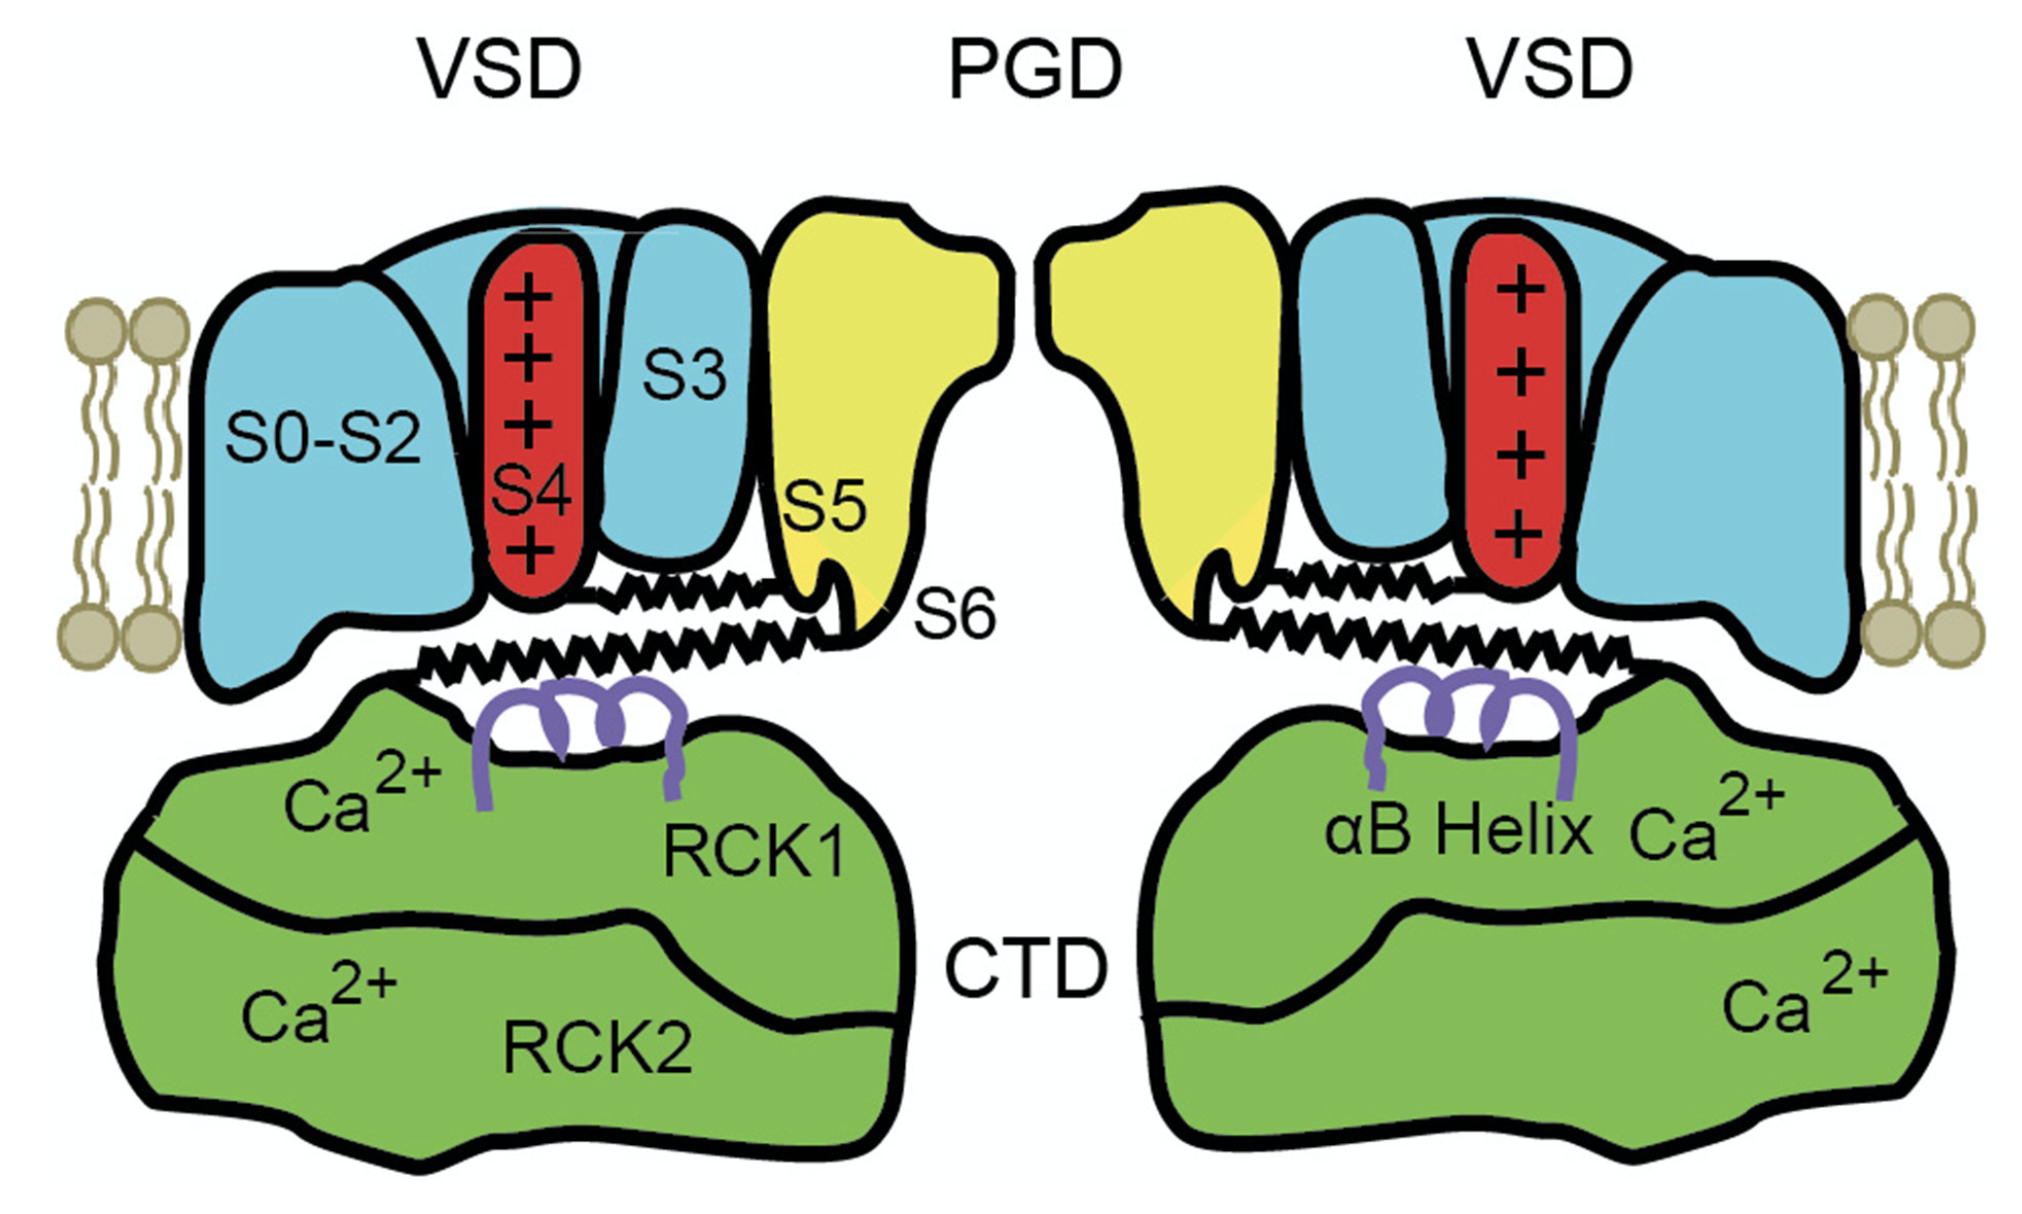
\includegraphics[width=.5\textwidth]{BK_Cartoon.png}
\end{figure}

Future studies:
\begin{itemize}
	\item Possibility of interaction between various sensors
	\item Agreement of 50-state DSM with macro current data
	\item Relaxation of the assumption of single $\ca$ binding site
\end{itemize}

\end{frame}

\begin{frame}
\begin{center}
\huge{THANK YOU}
\end{center}
\end{frame}


\begin{comment}
IMAGE REFERENCES:

Cell_Fluorescence: https://en.wikipedia.org/wiki/Neurotubule
\end{comment}


\end{document}